\chapter{Hauptkomponentenanalyse}   

Die Hauptkomponentenanalyse (engl.\ \emph{Principal Component Analysis}, PCA) ist ein Verfahren zur Dimensionsreduktion von Daten.
Genauer: Es handelt sich um eine Methode, um komplexe Daten auf ihr Wesentliches zu reduzieren, was eine Weiterverarbeitung und Visualisierung erleichtert.

In diesem Kapitel wird zunächst die Intuition hinter der PCA erläutert, bevor der mathematische Hintergrund und insbesondere die Verbindung zur Singulärwertzerlegung beschrieben wird.
Abschließend betrachten wir ein konkretes Anwendungsbeispiel und veranschaulichen dieses mithilfe der Programmiersprache \texttt{Python}.

\section{Intuition der PCA}
Angenommen, beim Familienessen käme die Frage auf, welche der mitgebrachten Weine sich am ähnlichsten sind. 
Um diese Frage zu beantworten, überlegt sich die Familie verschiedene Merkmale und ordnet jedem Wein für jedes Merkmal Zahlen zwischen \num{-3} und \num{3} zu.
Dadurch können die Weine als Punkte im Raum bezüglich der verschiedenen Werte dargestellt und anschließend analysiert werden, welche Weine sich gruppieren, also sich ähneln. 

In \zcref{fig:pcadim}, zu finden im \zcref{appen}, wird dies für verschiedene \(n \coloneqq \emph{Anzahl der Merkmale}\) verdeutlicht. 

Das Problem wird schnell ersichtlich:
Eine visuelle Interpretation ist zwar möglich, allerdings nur im niedrig-dimensionalen Raum, für eine größere Anzahl an Merkmalen (Dimensionen) besteht die Notwendigkeit, die Anzahl zu reduzieren.
Diese Dimensionsreduktion stellt in vielen Fällen auch unabhängig von der visuellen Interpretation eine sinnvolle Maßnahme dar.
In Bezug auf unser Beispiel bestehe die Möglichkeit, dass \enquote{Alkoholgehalt} und \enquote{Schwere} stark korrelieren und somit redundant für eine Rekonstruktion der Weine sind.
Eine andere Möglichkeit zur Reduzierung der Merkmale ist dadurch gegeben, dass gewisse Merkmale wenig Informationen über die Charakteristiken der Weine enthalten, wie beispielsweise die Flaschenform oder die Fließgeschwindigkeit.

Die Hauptkomponentenanalyse konstruiert neue, unkorrelierte Richtungen, die sich als Linearkombinationen aus den bestehenden Merkmalen zusammensetzen.
Dadurch könnten beispielsweise \enquote{Alkoholgehalt} und \enquote{Schwere} zu einer neuen \emph{Hauptrichtung} zusammengefasst werden.
Anschließend werden die Weine auf den durch diese Richtung definierten Unterraum projiziert.
Die projizierten Koordinaten entlang dieser neuen Achse ergeben die erste \emph{Hauptkomponente} (PC1).
Der Unterschied zwischen Hauptrichtung und Hauptkomponente wird am Ende der Intuition präzisiert.

Die Projektion wird in \zcref{fig:pca2d} veranschaulicht.
\begin{figure}[bt]
    \centering
    \begin{subfigure}{\textwidth}
        \centering
        \caption{}\label{fig:pca2d1}
        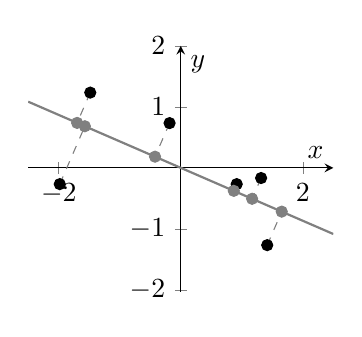
\begin{tikzpicture}[baseline]
        \begin{axis}[
            xlabel={\(x\)},
            ylabel={\(y\)},
            axis y line=center,
            axis x line=middle,
            axis equal,
            width=0.45\textwidth,
            xmin=-2.5,
            xmax=2.5
        ]
        \addplot[only marks,mark options={fill=black, color=black},domain=-2:2] coordinates {
            (1.4167,-1.2667)
            (-1.4833,1.2333)
            (1.3167,-0.1667)
            (-1.9833,-0.2667)
            (0.9167,-0.2667)
            (-0.1833,0.7333)                
        };
        \addplot[Gray, thick, domain=-2.5:2.5] {-0.4337*x};

        \addplot[only marks, mark options={fill=Gray, color=Gray}] coordinates {
            ( 1.65481157, -0.71762599)
            (-1.69867778,  0.73664903)
            ( 1.16912424, -0.50700271)
            (-1.57200891,  0.68171777)
            ( 0.86894276, -0.37682593)
            (-0.42195053,  0.18298317)
        };
        \addplot[dashed, gray] coordinates {
            (1.4167, -1.2667) ( 1.65481157, -0.71762599)
        };
        \addplot[dashed, gray] coordinates {
            (-1.4833, 1.2333) (-1.69867778,  0.73664903)
        };
        \addplot[dashed, gray] coordinates {
            (1.3167, -0.1667) ( 1.16912424, -0.50700271)
        };
        \addplot[dashed, gray] coordinates {
            (-1.9833, -0.2667) (-1.57200891,  0.68171777)
        };
        \addplot[dashed, gray] coordinates {
            (0.9167, -0.2667) (0.86894276, -0.37682593)
        };
        \addplot[dashed, gray] coordinates {
            (-0.1833, 0.7333) (-0.42195053,  0.18298317)  
        };
        \end{axis}
    \end{tikzpicture}
        \hspace{20pt}
        \begin{tikzpicture}[baseline]
    \begin{axis}[
        xlabel={\(PC1\)},
        ylabel={},
        axis y line=center,
        axis x line=middle,
        axis equal,
        ytick=\empty,
        width=0.45\textwidth,
        xmin=-2.5,
        xmax=2.5
    ]
    \addplot[only marks, mark options={fill=black, color=black}] coordinates {
        ( 1.803, 0)
        (-1.849, 0)
        ( 1.279, 0)
        (-1.697, 0)
        ( 0.928, 0)
        (-0.469, 0)
    };


    \end{axis}
\end{tikzpicture}
    \end{subfigure}
    \begin{subfigure}{\textwidth}
        \centering
        \caption{}\label{fig:pca2d2}
        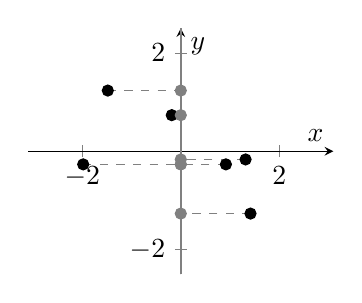
\begin{tikzpicture}[baseline]
    \begin{axis}[
        xlabel={\(x\)},
        ylabel={\(y\)},
        axis y line=center,
        axis x line=middle,
        axis equal,
        width=0.45\textwidth,
        xmin=-2.5,
        xmax=2.5
    ]
    \addplot[only marks,mark options={fill=black, color=black},domain=-2:2] coordinates {
        (1.4167,-1.2667)
        (-1.4833,1.2333)
        (1.3167,-0.1667)
        (-1.9833,-0.2667)
        (0.9167,-0.2667)
        (-0.1833,0.7333)                
    };
    \addplot[Gray, thick, domain=-2.5:2.5] ({0}, x);

    \addplot[only marks, mark options={fill=Gray, color=Gray}] coordinates {
        (0,-1.2667)
        (0,1.2333)
        (0,-0.1667)
        (0,-0.2667)
        (0,-0.2667)
        (0,0.7333)
    };
    \addplot[dashed, gray] coordinates {
        (1.4167, -1.2667) (0,-1.2667)
    };
    \addplot[dashed, gray] coordinates {
        (-1.4833, 1.2333) (0,1.2333)
    };
    \addplot[dashed, gray] coordinates {
        (1.3167, -0.1667) (0,-0.1667)
    };
    \addplot[dashed, gray] coordinates {
        (-1.9833, -0.2667) (0,-0.2667)
    };
    \addplot[dashed, gray] coordinates {
        (0.9167, -0.2667) (0,-0.2667)
    };
    \addplot[dashed, gray] coordinates {
        (-0.1833, 0.7333) (0,0.7333)  
    };
    \end{axis}
\end{tikzpicture}
        \hspace{20pt}
        \begin{tikzpicture}[baseline]
    \begin{axis}[
        xlabel={\(PC1\)},
        ylabel={},
        axis y line=center,
        axis x line=middle,
        axis equal,
        ytick=\empty,
        width=0.45\textwidth,
        xmin=-2.5,
        xmax=2.5
    ]
    \addplot[only marks, mark options={fill=black, color=black}] coordinates {
        (-1.2667,0)
        (1.2333,0)
        (-0.1667,0)
        (-0.2667,0)
        (-0.2667,0)
        (0.7333,0)
    };


    \end{axis}
\end{tikzpicture}
    \end{subfigure}
    \caption{Projektionen im zweidimensionalen Raum}\label{fig:pca2d}
\end{figure}
Der Unterschied zwischen \zcref{fig:pca2d1} und \zcref{fig:pca2d2} zeigt folgendes Problem auf:
Wie kann die neue Richtung optimal gewählt werden, sodass unsere Daten trotz der Dimensionsreduktion so originalgetreu wie möglich rekonstruiert werden können?
Dafür gibt es zwei alternative, aber äquivalente, Formulierungen:
\begin{enumerate}
    \item Die Richtung wird so konstruiert, dass ein Minimum an Informationen verloren wird.
    \item Die Richtung wird so konstruiert, dass eine maximale Varianz erhalten bleibt.
\end{enumerate}
Eine Äquivalenz dieser beiden Aussagen kann durch den Satz des Pythagoras hergeleitet werden, indem das rechtwinklige Dreieck zwischen einem Punkt, dessen Projektion und dem Ursprung betrachtet wird. 
Wird der Informationsverlust (Distanz zwischen der Projektion und dem Original) minimiert, maximiert sich die Varianz (Abstand zum Ursprung).
Es sei angemerkt, dass dafür von einer Zentrierung der Daten ausgegangen wird, also von einem Mittelwert gleich null.

Mit diesem Hintergrund wird intuitiv ersichtlich, dass \zcref{fig:pca2d1} im Vergleich zu \zcref{fig:pca2d2} vorzuziehen ist, was sich im Ergebnis widerspiegelt, in dem die räumliche Verteilung im Wesentlichen erhalten bleibt.

In vielen mathematischen Texten erfolgt keine klare Differenzierung zwischen den Begriffen Hauptrichtung und Hauptkomponente.
Stattdessen wird der Begriff Hauptkomponente häufig synonym für beide verwendet.
In dieser Arbeit definieren wir die erste Hauptrichtung als den Einheitsvektor, der den eindimensionalen Unterraum aufspannt, auf den die Daten projiziert werden.
Die erste Hauptkomponente bezeichnet die projizierten Koordinaten der Datenpunkte entlang dieser Hauptrichtung.
In höheren Dimensionen wird die zweite Hauptrichtung so gewählt, dass sie orthogonal zur ersten Hauptrichtung liegt und die verbleibende Varianz maximiert.
Dies kann beliebig fortgesetzt werden, die PCA besitzt allerdings die nützliche Eigenschaft, dass die Hauptrichtungen nach \enquote{Wichtigkeit} sortiert sind, also die ersten Richtungen bereits den Großteil der Varianz erklären.
Eine genauere Erläuterung dieser Aussage wird dabei in der folgenden mathematischen Herleitung gegeben.

\section{Mathematische Herleitung}
Bevor die vorangegangenen Überlegungen formalisiert werden können, rekapitulieren wir durch \zcref{rep:proj} die Formel der orthogonalen Projektion.
\begin{repitition}\label{rep:proj}
    Sei \(n \in \N\) und \(u,x \in \R^{n}\) mit \(\norm{u} = 1\).  \\
    Dann ist der orthogonal projizierte Vektor \(\operatorname{proj}_{u}(x)\) von \(x\) auf \(u\) gegeben durch
    \begin{equation*}
        \operatorname{proj}_{u}(x) = \langle x,u \rangle u = (x^{T}u)u.
    \end{equation*}     
\end{repitition}
Das Ziel der Herleitung in diesem Abschnitt wird durch \zcref{app:pca} zusammengefasst.
\begin{application}[PCA]\label{app:pca}
    Seien \(n,d \in \N\) und  
    \begin{equation*}
        X = 
        \big[
            \begin{matrix}
                x_1 \dots x_d
            \end{matrix}    
        \big] \in \R^{n \times d}
    \end{equation*} 
    eine standardisierte\footnote{Siehe \hyperref[itm:pca1]{Schritt 1} im Beweis} Datenmatrix, die \(d\) Merkmale über \(n\) Objekte hinweg speichert und
    \begin{equation*}
        \R^{d} \ni x^{(i)} \coloneqq X_{i,:} \quad \text{für } i \in \{1,\ldots,n\},
    \end{equation*}
    die \(i\)-te (transponierte) Zeile von \(X\), also ein Datenpunkt.     \\
    Bei der Projektion der Daten auf \(\R^{k}\) mit \(\N \ni k < d\) wird die Basis dieses Unterraums durch die ersten \(k\) Hauptrichtungen \(u_{j}\) für \(j \in \{1,\ldots,k\}\) gegeben, die den Eigenvektoren der Matrix \(\frac{1}{n}X^{T}X\) entsprechen, sortiert in absteigender Reihenfolge der zugehörigen Eigenwerte.
\end{application}
\begin{proof}
    Der Beweis orientiert sich zum Großteil an~\cite[S.~166-169]{ngMachineLearningCS2292023} und~\cite{hsuMachineLearningTheory2016}.
    \begin{enumerate}[wide,label=\underline{Schritt \arabic*}.]
        \item\label{itm:pca1} Vorbereitung der Daten:\\    
        Wir standardisieren zunächst \(X\), indem 
        \begin{equation*}
            x_{j}^{(i)} \leftarrow \frac{x_{j}^{(i)}-\mu_j}{\sigma_j} \quad \text{für alle } j \in \{1,\ldots,d\},
        \end{equation*}  
        wobei 
        \begin{equation*}
            \mu_j = \frac{1}{n}\sum_{i=1}^{n}x_{j}^{(i)}, \quad \sigma_{j}^{2} = \frac{1}{n}\sum_{i=1}^{n}{(x_{j}^{(i)} - \mu_{j})}^{2}
        \end{equation*}
        jeweils die Mittelwerte, bzw.\ die Varianzen der einzelnen Merkmale, also der Spalten sind.
        Durch die Subtraktion des Mittelwerts werden die Daten um den Ursprung zentriert.
        Die Division durch die Standardabweichung verhindert Ungenauigkeiten, die aufgrund unterschiedlicher Skalen der Merkmale entstehen könnten.
        Falls Merkmal A beispielsweise das Bruttoinlandsprodukt und Merkmal B die Geburtenrate verschiedener Länder darstellt, wird dadurch eine Vergleichbarkeit gewährleistet.
        In den folgenden Berechnungen wird eine Standardisierung angenommen und weiterhin mit \(X\) gearbeitet.
        \item\label{itm:pca2} Herleitung für \(k=1\):\\
        Es sei daran erinnert, dass die erste Hauptrichtung der Richtung entspricht, die die Varianz der Projektion maximiert.
        Dafür wird zunächst der Mittelwert \(\mu_{\operatorname{proj}}\) der projizierten Vektoren berechnet:
        \begin{equation*}
            \mu_{\operatorname{proj}} = \frac{1}{n}\sum_{i=1}^{n}\big(x^{{(i)}^{T}}u\big)u = \left({\left(\frac{1}{n}\sum_{i=1}^{n}x^{(i)}\right)}^{T}u\right)u = \symbf{0},
        \end{equation*}
        da durch die Standardisierung der Spaltenmittelwert für jede Spalte von \(X\) null beträgt, wodurch
        \begin{equation*}
            \sum_{i=1}^{n}x^{(i)} = \symbf{0}.
        \end{equation*}
        Die Entfernung (Abweichung) vom Mittelwert, also dem Ursprung, für einen beliebigen Vektor \(x^{(i)}\) beträgt
        \begin{equation*}
            \norm{\operatorname{proj}_{u}\big(x^{(i)}\big)} = \norm{\big(x^{{(i)}^{T}}u\big)u} =  \abs{\big(x^{{(i)}^{T}}u\big)}\norm{u} = \abs{x^{{(i)}^{T}}u}.
        \end{equation*}
        Damit ist die Varianz der projizierten Punkte gegeben durch 
        \begin{align*}
            \frac{1}{n}\sum_{i=1}^{n}{\big(x^{{(i)}^{T}}u\big)}^{2} &= \frac{1}{n}\sum_{i=1}^{n}x^{{(i)}^{T}}ux^{{(i)}^{T}}u \\
            &= \frac{1}{n}\sum_{i=1}^{n}u^{T}x^{(i)}x^{{(i)}^{T}}u \qquad (\text{Skalarprodukt kommutativ})\\
            &= u^{T}\left(\frac{1}{n}\sum_{i=1}^{n}x^{(i)}x^{{(i)}^{T}}\right)u
        \end{align*}
        Definiere 
        \begin{equation*}
            \Sigma \coloneqq \frac{1}{n}\sum_{i=1}^{n}x^{(i)}x^{{(i)}^{T}} \in \R^{d \times d}.
        \end{equation*}
        Bei standardisierten Daten ist diese Matrix als \emph{Kovarianzmatrix} bekannt, in unserem Fall ist sie die Kovarianzmatrix der verschiedenen Merkmale.
        Damit haben wir das Ziel der Herleitung auf folgendes Optimierungsproblem reduziert:
        \begin{alignat*}{2}
            &\!\max \qquad &&u^{T} \Sigma u, \\
            &\text{u.d.B.}  &&\norm{u}=1.
        \end{alignat*}
        Dieses Optimierungsproblem wird in der Literatur meist mithilfe von Lagrange-Multiplikatoren gelöst.
        In dieser Arbeit werden wir einen anderen Ansatz verfolgen und mit dem, im vorherigen Kapitel bewiesenen, Spektralsatz (\zcref{spec}) vorgehen.
        Beachte dafür zunächst, dass \(\Sigma\) symmetrisch ist: 
        \begin{equation*}
            \Sigma^{T} = {\left(\frac{1}{n}\sum_{i=1}^{n}x^{(i)}x^{{(i)}^{T}}\right)}^{T} = \frac{1}{n}\sum_{i=1}^{n}{\left(x^{(i)}x^{{(i)}^{T}}\right)}^{T} = \Sigma.
        \end{equation*}
        Dadurch ist die Voraussetzung für den Spektralsatz erfüllt, womit 
        \begin{equation*}
            \Sigma = R \Lambda R^{T}
        \end{equation*}
        für orthogonales \(R =
        \big[
            \begin{matrix}
                r_{1}\ldots r_{d}
            \end{matrix}
        \big] \in \R^{d \times d}\) und diagonales \(\Lambda = \operatorname{diag}(\lambda_1,\ldots,\lambda_d)\) mit \(\lambda_1 \geq \cdots \geq \lambda_d\).
        Für \(w \coloneqq R^{T}u\) gilt dann
        \begin{equation*}
            u^{T}\Sigma u = u^{T}R \Lambda R^{T} u = w^{T}\Lambda w = w^{T}
            \begin{bmatrix}
                \lambda_1 w_{1} \\
                \vdots \\
                \lambda_d w_{d}
            \end{bmatrix}
            =\sum_{i=1}^{d}\lambda_{i}w_{i}^{2}.
        \end{equation*}
        Nach Bedingung gilt \(\norm{u}=1\), womit:
        \begin{equation*}
            \norm{w} = \norm{R^{T}u} = \sqrt{\langle R^{T}u,R^{T}u \rangle} = \sqrt{u^{T}RR^{T}u} = \norm{u} = 1.
        \end{equation*} 
        Da 
        \begin{equation*}
            \sum_{i=1}^{d}\lambda_{i}w_{i}^{2} = \lambda_{1}w_{1} + \lambda_{2}w_{2} + \cdots + \lambda_{d}w_{d}
        \end{equation*}
        und \(\lambda_1 \geq \cdots \geq \lambda_d\) wird der Ausdruck maximiert für \(w = \symbf{e}_{1}\).
        Es folgt
        \begin{equation*}
            u = Rw = R\symbf{e}_{1} = r_{1},
        \end{equation*}
        womit \(u\) nach \zcref{cor:spec} gleich dem zugehörigen Eigenvektor zum größten Eigenwert von \(\Sigma\) ist
    \item Herleitung für beliebiges \(k\) mit vollständiger Induktion über \(k\):\\
    \emph{Induktionsanfang}. Gegeben durch \hyperref[itm:pca2]{Schritt 2}.\\
    \emph{Induktionshypothese}. Angenommen die ersten \(k-1\) Eigenvektoren \(u_{1},\ldots,u_{k-1}\) von \(\Sigma\) maximieren die Varianz der Projektion.\\
    \emph{Induktionsschritt}. Wir wollen zeigen, dass 
    \begin{equation*}
        \frac{1}{n}\sum_{j=1}^{k}\sum_{i=1}^{n}{(x^{{(i)}^{T}}u_{j})}^{2}
    \end{equation*}
    maximiert wird für \(u_{k} = r_{k}\).
    Betrachte dafür
    \begin{equation*}
        \frac{1}{n}\sum_{j=1}^{k}\sum_{i=1}^{n}{(x^{{(i)}^{T}}u_{j})}^{2} = \underbrace{\frac{1}{n}\sum_{j=1}^{k-1}\sum_{i=1}^{n}{(x^{{(i)}^{T}}u_{j})}^{2}}_{A} + \underbrace{\frac{1}{n}\sum_{i=1}^{n}{(x^{{(i)}^{T}}u_{k})}^{2}}_{B}.
    \end{equation*}
    Nach Induktionshypothese ist \(A\) maximal für \(u_{1}=r_{1},u_{2}=r_{2},\ldots,u_{k-1}=r_{k-1}\). 
    Um \(B\) zu maximieren, wird analog zu \hyperref[itm:pca2]{Schritt 2} vorgegangen.
    Es wird das Optimierungsproblem
    \begin{alignat*}{2}
        &\!\max \qquad &&u_{k}^{T} \Sigma u_{k}, \\
        &\text{u.d.B.}  &&\norm{u_{k}}=1, \\   
        &&& \langle u_{k},u_{i} \rangle = 0 \quad \text{für alle } i \in \{1,\ldots,k-1\},    
    \end{alignat*}
    aufgestellt mit zusätzlicher Orthogonalitätsbedingung.
    Anschließend kann, mithilfe der zusätzlichen Eigenschaft, dass Eigenvektoren zu verschiedenen Eigenwerten bei symmetrischen Matrizen orthogonal sind (\zcref{rem:orth}), das Optimierungsproblem durch \(u_{k} = r_{k}\) gelöst werden, womit der Beweis abgeschlossen ist.
\end{enumerate}
\end{proof}

\section{Verbindung zur SVD}
